% !TeX spellcheck = es_ES
\section{Solución del problema}

\subsection{Carga de datos OSM y ARESEP}
Para la carga de datos de la OSM y ARESEP, se podía haber hecho uso de herramientas como osm2pgsql pero se optó por utilizar un plugin en QGIS (OSMDownloader) para descargar el archivo y utilizar al mismo QGIS para convertirlo a geojson menos cantidad de datos debido a las limitaciones del servidor ya mencionadas anteriormente.

De esta forma entonces se podía utilizar la herramienta org2org y de igual forma, para simplificar procesos y hacerlo todo en base a este estándar de utilizar QGIS como medio para descargar los datos y pasarlos a geojson, se procedió a hacer lo mismo con los datos de la ARESEP.

\subsection{Base de datos}
La base de datos sigue el siguiente diagrama:
\begin{center}
	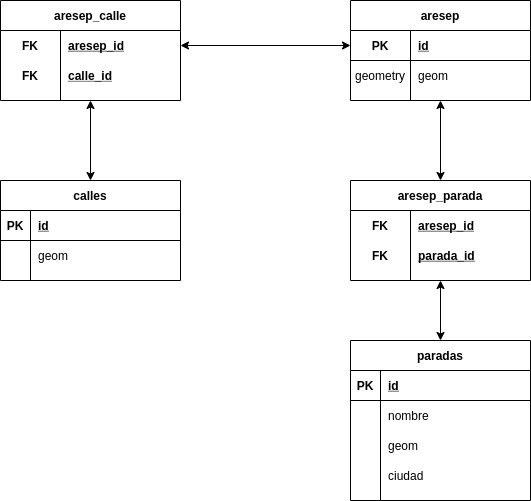
\includegraphics[scale=.65]{imagenes/diagram_db.png}
\end{center}

Para profundizar un poco más en los detalles del mismo, la tabla intermedia entre $aresep$ y $paradas$ es la que permite reducir la cantidad de datos a comparar posteriormente para hacer el llenado de la tabla de $aresep\_calle$.
Por otra parte, si por alguna razón para llegar a $X$ parada no existe una ruta oficial de la ARESEP o calle conectada (por dirección de la calle o por no estar conectada) entonces se podría conocer cuales paradas se encuentran en la misma ciudad y tomarlas como que comparten ruta y que esto se pueda llegar a representar a la hora de construir la topología y aplicar el dijkstra.

La función de la tabla $aresep\_calle$ es simplemente, ayudar a relación calle con $aresep$ pero más que eso está pensada en reducir la creación de la topología y posteriormente reducir el dijkstra.

Algo a recalcar también es que los datos descargados de OSM son 15 mill calles (sin filtros) y están en 4326 y las del ARESEP en 5367, por lo que para evitar estar haciendo transformaciones de datos y al ser la tabla del ARESEP menor en cantidad de datos, se le agrega una columna geométrica con los datos en 5367.

\subsection{Backend}
Se utilizó nodejs debido a que es una herramienta fácil correr en otras computadores y que ya lleva incorporado dentro del conjunto de archivos las versiones y datos necesarios para correr.

\subsection{Frontend}
Para el frontend se utiliza svelte por el factor reactivo y peso del framework y leaflet. 

\subsection{Indices}
En cuanto a los \textbf{indices} en las tablas se tienen a GIST y SPGIST; según el usuario \textcite{geozelot} menciona que SPGIST necesita menos espacio que que GIST por lo que es algo a considerar, además \textcite{Ramsey} menciona  que SPGIST supera a GIST cuando se procesan datos que no se superponen sobre otros (caso de las calles), por lo que para las calles se estaría utilizando SPGIST y para las rutas del ARESEP que suelen pasar varias por el mismo punto, se estaría utilizando GIST.

\subsection{Creación de la topología}
La creación de la topología se mantuvo a como se mencionó en el análisis del problema.

\subsection{Ruta más corta}
Para la ruta más corta se tuvo que hacer modificaciones sobre la capa del OSM y ARESEP, en el OSM para que calles que no intersecaban lo pudiesen hacer, esto mediante cortes o ligeras extensiones de las rutas, esto a pesar de que visualmente parecían tener conexión.

Por otra parte no se hizo uso del análisis de paradas por ciudad y no se sigue un ruteo estricto por rutas oficiales de parada a parada, si no por calles por donde pasan las rutas oficiales, esto porque algunas rutas se salían de las calles descargadas.

En cuanto a la modificación de las rutas del ARESEP, esto se hizo porque distaban mucho de las calles por donde se notaba que debían transitar, un ejemplo es la siguiente imagen donde se observa que las rutas del ARESEP incluso pasan sobre edificios.

\begin{center}
	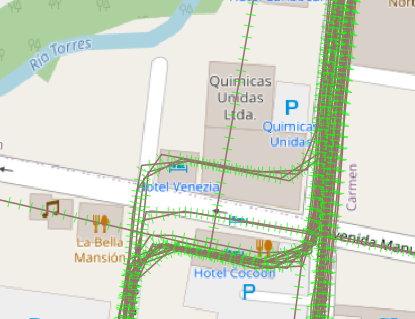
\includegraphics[scale=.65]{imagenes/ruta_aresep.png}
\end{center}

\newpage
